\section{Diagnostik, sensitivitas dan kekuatan bukti}\label{sec:diagnostics}
\subsection{Penyaringan level dan diagnostik dibedakan}
Sebanyak 95 dari 176 model utama menolak hipotesis tidak ada hubungan level menurut F dan t pada lima persen. Setelah joint-X, akar, risiko integrasi orde dua dan derajat bebas dipertimbangkan, 62 memenuhi syarat level operasional. Sebanyak 28 sekaligus tidak ditolak pada penyaringan residual dan stabilitas yang digunakan. Angka terakhir tidak berarti hanya 28 model benar, atau bahwa model lain tidak memberi informasi. Ia menunjukkan konsekuensi satu himpunan aturan yang dibuat transparan.

Diagnostik meliputi Breusch--Godfrey untuk korelasi serial, Breusch--Pagan untuk heteroskedastisitas, RESET untuk indikasi bentuk fungsi, Jarque--Bera untuk normalitas, ARCH, serta CUSUM dan CUSUMSQ untuk stabilitas. Normalitas bukan syarat universal konsistensi OLS, dan penolakan normalitas tidak mempunyai arti yang sama dengan penolakan kestabilan parameter. Penggabungan semuanya sebagai flag bersih adalah pilihan penyaringan yang konservatif. Pembaca tetap perlu melihat jenis penolakan, bukan hanya satu status akhir.

Tidak ditolaknya diagnostik juga bukan bukti bahwa asumsi pasti benar. Daya uji dapat rendah pada sampel kecil atau ketika banyak parameter diestimasi. Hasil residual yang tampak baik belum menyelesaikan endogenitas kurs, pemilihan variabel, maupun salah pengukuran. Probabilitas kecil menunjukkan ketidakcocokan data dengan hipotesis nol di bawah asumsi uji, bukan probabilitas bahwa hipotesis nol itu benar.

\subsection{Stabilitas dan pemeriksaan independen}
CUSUM utama diekspor langsung melalui \texttt{estat sbcusum} dari UECM dengan lag dan sampel terpilih \cite{stata}. Maksimum lintasan direkonsiliasi terhadap statistik tersimpan untuk seluruh 176 model utama. Pada matriks awal full rank, konstruksi independen juga diwajibkan cocok dalam toleransi numerik.

Dua model kelompok Australia, modal dan konsumsi NARDL, mempunyai matriks awal yang belum full rank. Prosedur independen menunda inisialisasi sampai full rank, sehingga berbeda dari Stata. Lintasan resmi Stata dipertahankan, perbedaannya dicatat, dan kedua model diberi caveat. Kasus tersebut berbeda dari model bilateral Australia yang dibahas pada hasil utama.

CUSUMSQ memakai referensi Gaussian Monte Carlo dengan 19.999 simulasi dan seed tetap. Band simultan referensinya hanya berlaku dalam konstruksi diagnostik tersebut, tidak mengubah band respons dinamis menjadi simultan. Perkiraan probabilitas Monte Carlo bersifat aproksimasi dan tidak diklaim sebagai tabel persis paper. Agregat perdagangan Indonesia memberi catatan CUSUMSQ, sedangkan Australia tidak ditolak dalam penyaringan utama.

\begin{figure}[!htbp]\centering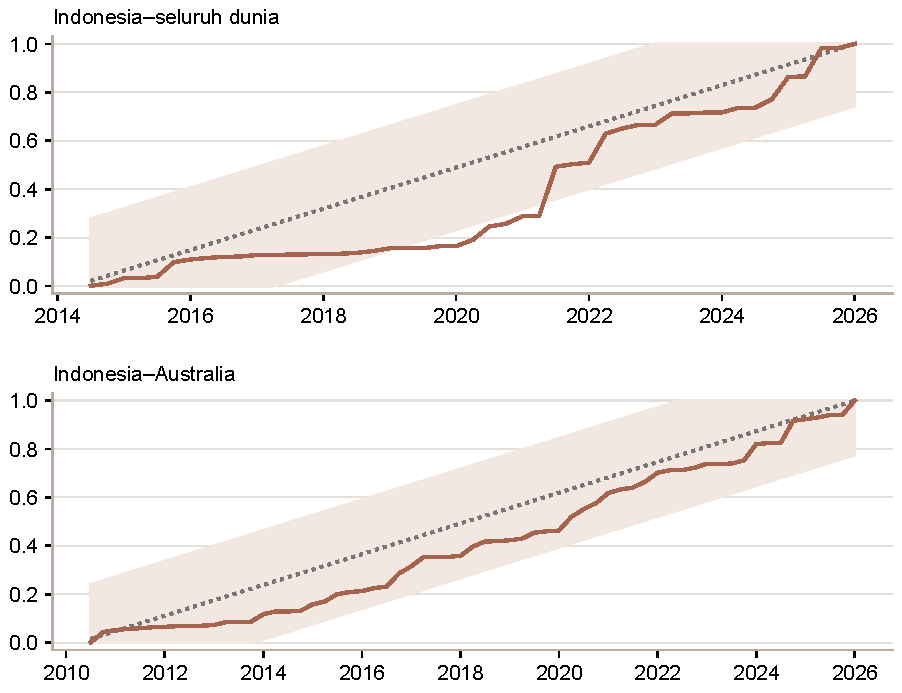
\includegraphics[width=\linewidth]{assets/stability.pdf}
\caption{CUSUMSQ NARDL agregat Indonesia dan Indonesia--Australia. Area menunjukkan band referensi simulasi; garis titik adalah lintasan ekspektasi. Ini diagnostik stabilitas, bukan band ketidakpastian efek kurs.}\label{fig:stability}
\end{figure}

Seluruh model juga diperiksa melalui ekuivalensi residual persamaan level dan ECM serta prediksi OLS independen. Pemeriksaan numerik itu lulus. Maknanya adalah bahwa perhitungan yang dilakukan konsisten, bukan bahwa semua asumsi ekonomi dan inferensinya telah terbukti.

\subsection{Ketahanan terhadap lag, harga dan sumber}
Pada ARDL, arah negatif komoditas total dan energi/tambang tetap muncul ketika cap dipersempit menjadi dua serta ketika BCOM ditambahkan. Namun beberapa varian memiliki catatan diagnostik. NARDL belum memberikan koefisien depresiasi yang signifikan pada kelompok ini, dan dukungan level dapat berubah menurut cap. Ketahanan tanda pada subset model linier karena itu tidak cukup untuk menyatakan hasil tahan terhadap seluruh spesifikasi.

\begin{table}[!htbp]\centering
\caption{Pembanding ARDL komoditas Indonesia--seluruh dunia}
{\small\setlength{\tabcolsep}{3pt}\renewcommand{\arraystretch}{1.15}
\begin{tabular}{p{0.08\linewidth}p{0.2\linewidth}p{0.08\linewidth}p{0.2\linewidth}p{0.15\linewidth}p{0.12\linewidth}}
\toprule
\textbf{Kel.} & \textbf{Varian} & \textbf{N} & \textbf{Koef. kurs} & \textbf{p} & \textbf{Status}\\
\midrule
G6 & Utama & 61 & -1,355 & \(<0{,}001\) & L+D\\
G6 & Cap 2 & 63 & -1,536 & \(<0{,}001\) & L+D\\
G6 & BCOM & 61 & -1,378 & \(<0{,}001\) & L\\
G7 & Utama & 61 & -2,040 & \(<0{,}001\) & L+D\\
G7 & Cap 2 & 63 & -2,222 & \(<0{,}001\) & L\\
G7 & BCOM & 61 & -2,305 & \(<0{,}001\) & L\\
\bottomrule
\end{tabular}
}\label{tab:sens}
\end{table}

BCOM adalah indeks luas, bukan harga setiap HS-6. Ia dapat bergerak bersama aktivitas global, harga energi dan kondisi keuangan yang juga berkaitan dengan kurs. Memasukkannya sebagai regressor membantu menilai apakah hasil berubah ketika satu kontrol harga ditambahkan; ia belum mengidentifikasi saluran kausal harga global. Interval klasik pada model yang menolak heteroskedastisitas juga perlu dinilai ulang sebelum digunakan untuk klaim yang kuat.

Sensitivitas lain meliputi perluasan window agregat 2006+, WPI India, dan keluarga FX GEM untuk Thailand, Vietnam dan Korea. Perubahan sumber dapat mengubah konsep harga, nilai kurs, dan kelengkapan window sekaligus. Sebagian perbandingan itu belum merupakan eksperimen satu perubahan pada sampel identik. Semua 340 sensitivitas dipertahankan dalam lampiran agar pembaca dapat melihat hasil yang tidak searah dengan baseline.

Tiga model NARDL India dengan BCOM tidak memiliki inferensi bounds finite-sample yang tersedia pada implementasi: komoditas total, energi/tambang, dan bahan baku/penolong. Ketiganya mempunyai 49 observasi dan 25--27 parameter. Koefisiennya tetap diestimasi; status bounds adalah tidak tersedia dan tidak dipakai sebagai dukungan level. Ketidaktersediaan inferensi tidak diubah menjadi keputusan menerima atau menolak kointegrasi.

\subsection{Bentuk J pada titik dan dukungan dua fase}
Agar penilaian grafik dapat ditelusuri, pemeriksaan titik dalam deck dan naskah menggunakan
\begin{equation}
 \min_{0\le h\le4}R_h^{J,-}<0,\qquad
 \frac{1}{9}\sum_{h=16}^{24}R_h^{J,-}>0.
 \label{eq:jvisual}
\end{equation}
Ini definisi visual-operasional: setidaknya satu pemburukan pada tahun pertama, termasuk impact, dan rerata positif pada bagian akhir horizon. Definisi tersebut bukan uji formal J-curve paper, bukan long-run limit, dan tidak dipraregistrasikan sebagai desain inferensi.

\begin{table}[!htbp]\centering
\caption{Pola J pada seluruh model utama}
{\small\setlength{\tabcolsep}{3pt}\renewcommand{\arraystretch}{1.15}
\begin{tabular}{p{0.18\linewidth}p{0.12\linewidth}p{0.15\linewidth}p{0.21\linewidth}p{0.23\linewidth}}
\toprule
\textbf{Model} & \textbf{Seri} & \textbf{J titik} & \textbf{J + L+D} & \textbf{Dua fase CI}\\
\midrule
ARDL & 88 & 10 & 1 & 0\\
NARDL & 88 & 24 & 5 & 2\\
\bottomrule
\end{tabular}
}\label{tab:j}
\end{table}

Pada titik estimasi terdapat sepuluh pola J ARDL dan 24 NARDL. Setelah syarat level dan diagnostik diperiksa, tersisa satu ARDL dan lima NARDL. Syarat tambahan bahwa sebagian fase awal mempunyai batas atas di bawah nol dan kuartal ke-24 mempunyai batas bawah di atas nol menghasilkan nol ARDL dan dua NARDL. Dua NARDL itu adalah modal Korea dan konsumsi AS.

Pencarian salah satu horizon awal masih menimbulkan pengujian berganda, sehingga dua kasus tersebut tidak menjadi uji simultan dua fase yang sah. Jumlah model yang bertumpang tindih juga tidak dapat dibaca sebagai frekuensi kejadian J-curve di populasi. Yang dapat dinyatakan adalah bahwa bukti interval lebih terbatas daripada kesan visual titiknya.

\subsection{Mengapa ARDL dan NARDL dapat berbeda}
NARDL menambah parameter dan membagi variasi kurs ke dua partial sums yang dapat berkorelasi kuat dengan tren aktivitas ekonomi. Ketepatan efek satu arah dapat turun, sementara hubungan yang dipaksakan simetris pada ARDL menjadi lebih presisi. AIC juga dapat memilih lag yang berbeda. Perbedaan keduanya tidak otomatis membuktikan salah satu model benar.

Pemilihan model sebaiknya tidak hanya didasarkan pada tanda yang disukai. Relevansi ekonomi, kesesuaian definisi, dukungan level, ketepatan, diagnostik dan sensitivitas harus diperiksa bersama. Pada data yang ada, ketidaksepakatan antara hasil komoditas linier dan nonlinear merupakan bagian dari temuan, bukan gangguan yang dihapus dari narasi.
